\documentclass[manuscript,screen]{acmart}


\IfFileExists{upquote.sty}{\usepackage{upquote}}{}
\IfFileExists{microtype.sty}{% use microtype if available
  \usepackage[]{microtype}
  \UseMicrotypeSet[protrusion]{basicmath} % disable protrusion for tt fonts
}{}
\makeatletter
\@ifundefined{KOMAClassName}{% if non-KOMA class
  \IfFileExists{parskip.sty}{%
    \usepackage{parskip}
  }{% else
    \setlength{\parindent}{0pt}
    \setlength{\parskip}{6pt plus 2pt minus 1pt}}
}{% if KOMA class
  \KOMAoptions{parskip=half}}
\makeatother

%%
%% This is file `sample-manuscript.tex',
%% generated with the docstrip utility.
%%
%% The original source files were:
%%
%% samples.dtx  (with options: `manuscript')
%% 
%% IMPORTANT NOTICE:
%% 
%% For the copyright see the source file.
%% 
%% Any modified versions of this file must be renamed
%% with new filenames distinct from sample-manuscript.tex.
%% 
%% For distribution of the original source see the terms
%% for copying and modification in the file samples.dtx.
%% 
%% This generated file may be distributed as long as the
%% original source files, as listed above, are part of the
%% same distribution. (The sources need not necessarily be
%% in the same archive or directory.)
%%
%%
%% Commands for TeXCount
%TC:macro \cite [option:text,text]
%TC:macro \citep [option:text,text]
%TC:macro \citet [option:text,text]
%TC:envir table 0 1
%TC:envir table* 0 1
%TC:envir tabular [ignore] word
%TC:envir displaymath 0 word
%TC:envir math 0 word
%TC:envir comment 0 0
%%
%%
%% The first command in your LaTeX source must be the \documentclass command.


% Options for packages loaded elsewhere
\PassOptionsToPackage{unicode}{hyperref}
\PassOptionsToPackage{hyphens}{url}
\PassOptionsToPackage{dvipsnames,svgnames,x11names}{xcolor}

\IfFileExists{bookmark.sty}{\usepackage{bookmark}}{\usepackage{hyperref}}

%% PANDOC PREAMBLE BEGINS


\providecommand{\tightlist}{%
  \setlength{\itemsep}{0pt}\setlength{\parskip}{0pt}}\usepackage{longtable,booktabs,array}
\usepackage{calc} % for calculating minipage widths
% Correct order of tables after \paragraph or \subparagraph
\usepackage{etoolbox}
\makeatletter
\patchcmd\longtable{\par}{\if@noskipsec\mbox{}\fi\par}{}{}
\makeatother
% Allow footnotes in longtable head/foot
\IfFileExists{footnotehyper.sty}{\usepackage{footnotehyper}}{\usepackage{footnote}}
\makesavenoteenv{longtable}
\usepackage{graphicx}
\makeatletter
\def\maxwidth{\ifdim\Gin@nat@width>\linewidth\linewidth\else\Gin@nat@width\fi}
\def\maxheight{\ifdim\Gin@nat@height>\textheight\textheight\else\Gin@nat@height\fi}
\makeatother
% Scale images if necessary, so that they will not overflow the page
% margins by default, and it is still possible to overwrite the defaults
% using explicit options in \includegraphics[width, height, ...]{}
\setkeys{Gin}{width=\maxwidth,height=\maxheight,keepaspectratio}
% Set default figure placement to htbp
\makeatletter
\def\fps@figure{htbp}
\makeatother
\newlength{\cslhangindent}
\setlength{\cslhangindent}{1.5em}
\newlength{\csllabelwidth}
\setlength{\csllabelwidth}{3em}
\newlength{\cslentryspacingunit} % times entry-spacing
\setlength{\cslentryspacingunit}{\parskip}
\newenvironment{CSLReferences}[2] % #1 hanging-ident, #2 entry spacing
 {% don't indent paragraphs
  \setlength{\parindent}{0pt}
  % turn on hanging indent if param 1 is 1
  \ifodd #1
  \let\oldpar\par
  \def\par{\hangindent=\cslhangindent\oldpar}
  \fi
  % set entry spacing
  \setlength{\parskip}{#2\cslentryspacingunit}
 }%
 {}
\usepackage{calc}
\newcommand{\CSLBlock}[1]{#1\hfill\break}
\newcommand{\CSLLeftMargin}[1]{\parbox[t]{\csllabelwidth}{#1}}
\newcommand{\CSLRightInline}[1]{\parbox[t]{\linewidth - \csllabelwidth}{#1}\break}
\newcommand{\CSLIndent}[1]{\hspace{\cslhangindent}#1}

\definecolor{mypink}{RGB}{219, 48, 122}
\makeatletter
\makeatother
\makeatletter
\makeatother
\makeatletter
\@ifpackageloaded{caption}{}{\usepackage{caption}}
\AtBeginDocument{%
\ifdefined\contentsname
  \renewcommand*\contentsname{Table of contents}
\else
  \newcommand\contentsname{Table of contents}
\fi
\ifdefined\listfigurename
  \renewcommand*\listfigurename{List of Figures}
\else
  \newcommand\listfigurename{List of Figures}
\fi
\ifdefined\listtablename
  \renewcommand*\listtablename{List of Tables}
\else
  \newcommand\listtablename{List of Tables}
\fi
\ifdefined\figurename
  \renewcommand*\figurename{Figure}
\else
  \newcommand\figurename{Figure}
\fi
\ifdefined\tablename
  \renewcommand*\tablename{Table}
\else
  \newcommand\tablename{Table}
\fi
}
\@ifpackageloaded{float}{}{\usepackage{float}}
\floatstyle{ruled}
\@ifundefined{c@chapter}{\newfloat{codelisting}{h}{lop}}{\newfloat{codelisting}{h}{lop}[chapter]}
\floatname{codelisting}{Listing}
\newcommand*\listoflistings{\listof{codelisting}{List of Listings}}
\makeatother
\makeatletter
\@ifpackageloaded{caption}{}{\usepackage{caption}}
\@ifpackageloaded{subcaption}{}{\usepackage{subcaption}}
\makeatother
\makeatletter
\@ifpackageloaded{tcolorbox}{}{\usepackage[many]{tcolorbox}}
\makeatother
\makeatletter
\@ifundefined{shadecolor}{\definecolor{shadecolor}{rgb}{.97, .97, .97}}
\makeatother
\makeatletter
\makeatother
%% PANDOC PREAMBLE ENDS

\setlength{\parindent}{10pt}
\setlength{\parskip}{0pt}

\hypersetup{
  pdftitle={IS415 Report},
  pdfauthor={Chen Hao Xian; Tan Wen Yang; Pierre Jean Michel},
  colorlinks=true,
  linkcolor={blue},
  filecolor={Maroon},
  citecolor={Blue},
  urlcolor={red},
  pdfcreator={LaTeX via pandoc, via quarto}}

%% \BibTeX command to typeset BibTeX logo in the docs
\AtBeginDocument{%
  \providecommand\BibTeX{{%
    Bib\TeX}}}

%% Rights management information.  This information is sent to you
%% when you complete the rights form.  These commands have SAMPLE
%% values in them; it is your responsibility as an author to replace
%% the commands and values with those provided to you when you
%% complete the rights form.
\setcopyright{acmcopyright}
\copyrightyear{2023}
\acmYear{}
\acmDOI{}

%% These commands are for a PROCEEDINGS abstract or paper.
\acmConference[]{}{}{}
\acmPrice{}
\acmISBN{}

%% Submission ID.
%% Use this when submitting an article to a sponsored event. You'll
%% receive a unique submission ID from the organizers
%% of the event, and this ID should be used as the parameter to this command.
%%\acmSubmissionID{123-A56-BU3}

%%
%% For managing citations, it is recommended to use bibliography
%% files in BibTeX format.
%%
%% You can then either use BibTeX with the ACM-Reference-Format style,
%% or BibLaTeX with the acmnumeric or acmauthoryear sytles, that include
%% support for advanced citation of software artefact from the
%% biblatex-software package, also separately available on CTAN.
%%
%% Look at the sample-*-biblatex.tex files for templates showcasing
%% the biblatex styles.
%%

%%
%% The majority of ACM publications use numbered citations and
%% references.  The command \citestyle{authoryear} switches to the
%% "author year" style.
%%
%% If you are preparing content for an event
%% sponsored by ACM SIGGRAPH, you must use the "author year" style of
%% citations and references.
%% Uncommenting
%% the next command will enable that style.
%%\citestyle{acmauthoryear}


%% end of the preamble, start of the body of the document source.
\begin{document}


%%
%% The "title" command has an optional parameter,
%% allowing the author to define a "short title" to be used in page headers.
\title{IS415 Report}

%%
%% The "author" command and its associated commands are used to define
%% the authors and their affiliations.
%% Of note is the shared affiliation of the first two authors, and the
%% "authornote" and "authornotemark" commands
%% used to denote shared contribution to the research.


  \author{Chen Hao Xian}
  
    \author{Tan Wen Yang}
  
    \author{Pierre Jean Michel}
  
            \affiliation{%
                  \institution{Singapore Management University}
                                  \city{Singapore}
                                  \country{Singapore}
                      }
      

%% By default, the full list of authors will be used in the page
%% headers. Often, this list is too long, and will overlap
%% other information printed in the page headers. This command allows
%% the author to define a more concise list
%% of authors' names for this purpose.
%\renewcommand{\shortauthors}{Trovato et al.}
%%  
%% The abstract is a short summary of the work to be presented in the
%% article.
\begin{abstract}
A clear and well-documented \LaTeX~document is presented as an article
formatted for publication by ACM in a conference proceedings or journal
publication. Based on the ``acmart'' document class, this article
presents and explains many of the common variations, as well as many of
the formatting elements an author may use in the preparation of the
documentation of their work.    
\end{abstract}

%%
%% The code below is generated by the tool at http://dl.acm.org/ccs.cfm.
%% Please copy and paste the code instead of the example below.
%%

%%
%% Keywords. The author(s) should pick words that accurately describe
%% the work being presented. Separate the keywords with commas.
\keywords{HDB Prices, Linear Regression, Geographically Weighted
Regression, Exploratory Data Analysis}


%%
%% This command processes the author and affiliation and title
%% information and builds the first part of the formatted document.
\maketitle

\setlength{\parskip}{-0.1pt}

\hypertarget{motivation}{%
\section{Motivation}\label{motivation}}

With the price of HDB resale flats seeing tremendous growth over the
years, and news such as "\textbf{HDB resale prices accelerate in Jan as
million-dollar deals surge by 42\%: SRX, 99.co"} \citep{ducky23} or
\href{https://www.straitstimes.com/singapore/housing/hdb-resale-prices-rise-23-in-q4-slowest-increase-in-2022\#:~:text=Resale\%20prices\%20grew\%20by\%2010.4,latest\%20round\%20of\%20property\%20curbs.}{\textbf{"HDB
resale prices rise 2.3\% in Q4, slowest increase in 2022"}}
\citep{ducky32}, Singaporeans face the ever-growing concern as to
whether or not they are paying a fair price for their flats. Given the
lack of accessibility to geographically weighted models, users may find
it difficult to assess what factors impact the resale price of an HDB
flat; indeed, current estimators often only consider linear
relationships between dependent and independent variables and fail to
include geographical predictors in their models, which may limit the
ability of one regression to explain HDB resale prices; however,
geographically weighted regressions provide a more sophisticated way to
model spatial heterogeneity by accounting for the unique characteristics
of different neighborhoods.

Despite the advantages of geographically weighted regressions, they can
be difficult for casual users without specialized skills to use
effectively. Thus, our research comes in handy to give the right tools
to Singaporeans as we aim to:

\begin{enumerate}
\def\labelenumi{\arabic{enumi}.}
\item
  Identify the most significant location-specific variables that affect
  the resale price of HDB flats in Singapore and quantify their impact
  on pricing using geographically weighted regression models. By
  analyzing the relationship between different amenities, such as rail
  stations, hawker centers, preschools, malls, and mosquito hotspots, we
  aim to determine which factors have the most significant explanatory
  power on HDB resale prices and which do not. It will provide valuable
  insights into the most important factors that homebuyers and sellers
  should consider when transacting in the HDB resale market.
\item
  Develop a user-friendly web application that leverages geographically
  weighted regression models to estimate the resale value of HDB flats
  in Singapore for a given area. By inputting location-specific
  variables such as proximity to rail stations, hawker centers,
  preschools, malls, and mosquito hotspots, users can receive an
  estimated resale value for their property. It will provide users with
  a more accurate estimation of the value of their property, which can
  help them make better decisions when selling or buying an HDB flat.
\item
  Promote transparency and reduce information asymmetry in the HDB
  resale market by providing an accessible and user-friendly tool for
  estimating resale values. By making geographically weighted regression
  models more accessible to the public, we hope to empower homeowners,
  buyers, and policymakers to make more informed decisions about the HDB
  resale market. It could ultimately lead to better outcomes for buyers
  and sellers and help policymakers make more informed decisions about
  housing affordability, urban planning, and education policy.
\end{enumerate}

\hypertarget{relevant-related-work}{%
\section{Relevant Related Work}\label{relevant-related-work}}

We will now discuss past research in the fields of hedonic housing price
models and the importance of geography in these models. We shall review
three pieces of work in the following paragraphs.

Our
\href{https://journals.sagepub.com/doi/abs/10.1177/0042098013492234?journalCode=usja}{first
article}, ``Spatial Heterogeneity in Hedonic House Price Models: The
Case of Austria.'' by M. Helbich, C. Leitner, and A. Kapusta,
investigates the spatial heterogeneity of housing prices in Austria by
using a hedonic pricing model. This statistical model estimates the
value of a property based on its attributes, size, location, and other
factors, such as proximity to different amenities (e.g., shopping malls
and parks). In this paper, the writers apply geographically weighted
regression (GWR) analysis to identify local spatial patterns of the
housing market and examine the spatial variability of the hedonic price
model coefficients. In their research, they deduce that the GWR approach
provides more accurate predictions of housing prices than traditional
regression methods, which assume spatial homogeneity of coefficients.
Their study revealed that housing prices are significantly influenced by
local characteristics of neighborhoods as accessibility, environment,
and social amenities, to name a few. Their paper suggests that the
spatial heterogeneity of housing prices is crucial to accurately model
and analyze the housing market, especially in geographically diverse
regions like Austria. In our case, we consider the paper's methodology
and insights valuable for our research as we plan to investigate the
spatial heterogeneity of housing prices in Singapore and identify local
factors that affect house prices.

The second work we will analyze is the
\href{https://services2.hdb.gov.sg/webapp/BB33RTIS/}{HDB Resale Flat
Prices} web application developed by the Housing Development Board of
Singapore. It provides a platform for users to access information on
past resale transactions of Housing and Development Board (HDB) flats in
Singapore. It allows users to search for resale transactions based on
various criteria, such as location, flat type, and transaction period.
This web application is the perfect example of what Singaporeans are
missing, a model that explains the relevancy of locational factors on
HDB resale price. Nonetheless, this web application still serves as a
relevant solution that offers insights into the Singapore housing market
and the attributes of HDB flats that may affect transaction prices. We
believe there is room for improvement in the functionalities the
platform offers. Through our research, we aim to explore ways to improve
the current system, perhaps by incorporating additional data sources and
applying advanced machine learning algorithms to provide an accurate and
valuable explanatory model of housing prices.

The last piece of reading we shall discuss is the
\href{https://towardsdatascience.com/predict-the-selling-price-of-hdb-resale-flats-50530391a845}{Medium
article} ``Predict the Selling Price of HDB Resale Flats'' by Jim Meng
Kok. It uses machine learning to predict the selling price of HDB resale
flats in Singapore. The author uses a dataset of HDB resale transactions
and applies a random forest regression model to predict the resale price
of HDB flats based on various features, including location, size, age,
and nearby amenities. The model achieves a high accuracy rate,
indicating that machine learning methods can effectively predict housing
prices. The article is relevant to the current research on housing
prices in Singapore as it highlights the importance of utilizing machine
learning techniques for predicting prices accurately. While the author
uses Python in his analysis, we still consider that the insights
provided in the article can be valuable for any researcher planning to
use other programming languages, as R. The findings suggest that
location and amenities play a significant role in determining housing
prices, which is consistent with previous research on the topic.

In conclusion, this section has reviewed three pieces of research
related to hedonic housing price models and the importance of geography
in these models. Overall, these studies emphasize the need to account
for location and amenities when modeling and analyzing housing prices
and highlight the potential of advanced techniques like geographically
weighted regression and machine learning to provide more accurate
predictions.\\

\hypertarget{design-framework}{%
\section{\texorpdfstring{\textbf{Design
Framework}}{Design Framework}}\label{design-framework}}

The primary parameter given to the ``\texttt{acmart}'' document class is
the \emph{template style} which corresponds to the kind of publication
or SIG publishing the work. This parameter is enclosed in square
brackets and is a part of the ``\texttt{documentclass}'' command:

\begin{verbatim}
  \documentclass[STYLE]{acmart}
\end{verbatim}

Journals use one of three template styles. All but three ACM journals
use the ``\texttt{acmsmall}'' template style:

\begin{itemize}
\tightlist
\item
  \texttt{acmsmall}: The default journal template style.
\item
  \texttt{acmlarge}: Used by JOCCH and TAP.
\item
  \texttt{acmtog}: Used by TOG.
\end{itemize}

The majority of conference proceedings documentation will use the
``\texttt{cmconf}'' template style.

\begin{itemize}
\tightlist
\item
  \texttt{acmconf}: The default proceedings template style.
\item
  \texttt{sigchi}: Used for SIGCHI conference articles.
\item
  \texttt{sigchi-a}: Used for SIGCHI ``Extended Abstract'' articles.
\item
  \texttt{sigplan}: Used for SIGPLAN conference articles.
\end{itemize}

\hypertarget{demostration---use-case}{%
\section{Demostration - Use Case}\label{demostration---use-case}}

In addition to specifying the \emph{template style} to be used in
formatting your work, there are a number of \emph{template parameters}
which modify some part of the applied template style. A complete list of
these parameters can be found in the \LaTeX~User's Guide.

Frequently-used parameters, or combinations of parameters, include:

\begin{itemize}
\tightlist
\item
  \texttt{anonymous,review}: Suitable for a ``double-blind'' conference
  submission. Anonymizes the work and includes line numbers. Use with
  the \texttt{\textbackslash{}acmSubmissionID} command to print the
  submission's unique ID on each page of the work.
\item
  \texttt{authorversion}: Produces a version of the work suitable for
  posting by the author.
\item
  \texttt{screen}: Produces colored hyperlinks.
\end{itemize}

This document uses the following string as the first command in the
source file:

\begin{verbatim}
  \documentclass[manuscript,screen,review]{acmart}
\end{verbatim}

\hypertarget{modifications}{%
\section{Modifications}\label{modifications}}

Modifying the template --- including but not limited to: adjusting
margins, typeface sizes, line spacing, paragraph and list definitions,
and the use of the \texttt{\textbackslash{}vspace} command to manually
adjust the vertical spacing between elements of your work --- is not
allowed.

\textbf{Your document will be returned to you for revision if
modifications are discovered.}

\hypertarget{discussionconclusion}{%
\section{\texorpdfstring{\textbf{Discussion/Conclusion}}{Discussion/Conclusion}}\label{discussionconclusion}}

The ``\texttt{acmart}'' document class requires the use of the
``Libertine'' typeface family. Your \TeX~installation should include
this set of packages. Please do not substitute other typefaces. The
``\texttt{lmodern}'' and ``\texttt{ltimes}'' packages should not be
used, as they will override the built-in typeface families.

\hypertarget{title-information}{%
\section{Title Information}\label{title-information}}

The title of your work should use capital letters appropriately -
\url{https://capitalizemytitle.com/} has useful rules for
capitalization. Use the ``\texttt{title}'' command to define the title
of your work. If your work has a subtitle, define it with the
``\texttt{subtitle}'' command. Do not insert line breaks in your title.

If your title is lengthy, you must define a short version to be used in
the page headers, to prevent overlapping text. The ``\texttt{title}''
command has a ``short title'' parameter:

\begin{verbatim}
  \title[short title]{full title}
\end{verbatim}

\hypertarget{opening---potential-future-work}{%
\section{\texorpdfstring{\textbf{Opening - Potential Future
Work}}{Opening - Potential Future Work}}\label{opening---potential-future-work}}

Each author must be defined separately for accurate metadata
identification. As an exception, multiple authors may share one
affiliation. Authors' names should not be abbreviated; use full first
names wherever possible. Include authors' e-mail addresses whenever
possible.

Grouping authors' names or e-mail addresses, or providing an ``e-mail
alias,'' as shown below, is not acceptable:

\begin{verbatim}
  \author{Brooke Aster, David Mehldau}
  \email{dave,judy,steve@university.edu}
  \email{firstname.lastname@phillips.org}
\end{verbatim}

The \texttt{authornote} and \texttt{authornotemark} commands allow a
note to apply to multiple authors --- for example, if the first two
authors of an article contributed equally to the work.

If your author list is lengthy, you must define a shortened version of
the list of authors to be used in the page headers, to prevent
overlapping text. The following command should be placed just after the
last \texttt{\textbackslash{}author\{\}} definition:

\begin{verbatim}
  \renewcommand{\shortauthors}{McCartney, et al.}
\end{verbatim}

Omitting this command will force the use of a concatenated list of all
of the authors' names, which may result in overlapping text in the page
headers.

The article template's documentation, available at
\url{https://www.acm.org/publications/proceedings-template}, has a
complete explanation of these commands and tips for their effective use.

Note that authors' addresses are mandatory for journal articles.

\hypertarget{rights-information}{%
\section{Rights Information}\label{rights-information}}

Authors of any work published by ACM will need to complete a rights
form. Depending on the kind of work, and the rights management choice
made by the author, this may be copyright transfer, permission, license,
or an OA (open access) agreement.

Regardless of the rights management choice, the author will receive a
copy of the completed rights form once it has been submitted. This form
contains \LaTeX~commands that must be copied into the source document.
When the document source is compiled, these commands and their
parameters add formatted text to several areas of the final document:

\begin{itemize}
\tightlist
\item
  the ``ACM Reference Format'' text on the first page.
\item
  the ``rights management'' text on the first page.
\item
  the conference information in the page header(s).
\end{itemize}

Rights information is unique to the work; if you are preparing several
works for an event, make sure to use the correct set of commands with
each of the works.

The ACM Reference Format text is required for all articles over one page
in length, and is optional for one-page articles (abstracts).

\hypertarget{ccs-concepts-and-user-defined-keywords}{%
\section{CCS Concepts and User-Defined
Keywords}\label{ccs-concepts-and-user-defined-keywords}}

Two elements of the ``acmart'' document class provide powerful taxonomic
tools for you to help readers find your work in an online search.

The ACM Computing Classification System ---
\url{https://www.acm.org/publications/class-2012} --- is a set of
classifiers and concepts that describe the computing discipline. Authors
can select entries from this classification system, via
\url{https://dl.acm.org/ccs/ccs.cfm}, and generate the commands to be
included in the \LaTeX~source.

User-defined keywords are a comma-separated list of words and phrases of
the authors' choosing, providing a more flexible way of describing the
research being presented.

CCS concepts and user-defined keywords are required for for all articles
over two pages in length, and are optional for one- and two-page
articles (or abstracts).

\hypertarget{sectioning-commands}{%
\section{Sectioning Commands}\label{sectioning-commands}}

Your work should use standard \LaTeX~sectioning commands:
\texttt{section}, \texttt{subsection}, \texttt{subsubsection}, and
\texttt{paragraph}. They should be numbered; do not remove the numbering
from the commands.

Simulating a sectioning command by setting the first word or words of a
paragraph in boldface or italicized text is \textbf{not allowed.}

\hypertarget{tables}{%
\section{Tables}\label{tables}}

The ``\texttt{acmart}'' document class includes the
``\texttt{booktabs}'' package --- \url{https://ctan.org/pkg/booktabs}
--- for preparing high-quality tables.

Table captions are placed \emph{above} the table.

Because tables cannot be split across pages, the best placement for them
is typically the top of the page nearest their initial cite. To ensure
this proper ``floating'' placement of tables, use the environment
\textbf{table} to enclose the table's contents and the table caption.
The contents of the table itself must go in the \textbf{tabular}
environment, to be aligned properly in rows and columns, with the
desired horizontal and vertical rules. Again, detailed instructions on
\textbf{tabular} material are found in the \LaTeX~User's Guide.

Immediately following this sentence is the point at which
Table~\ref{tbl-freq} is included in the input file; compare the
placement of the table here with the table in the printed output of this
document.

\hypertarget{tbl-freq}{}
\begin{longtable}[]{@{}ccl@{}}
\caption{\label{tbl-freq}Frequency of Special Characters}\tabularnewline
\toprule()
Non-English or Math & Frequency & Comments \\
\midrule()
\endfirsthead
\toprule()
Non-English or Math & Frequency & Comments \\
\midrule()
\endhead
Ø & 1 in 1,000 & For Swedish names \\
\(\pi\) & 1 in 5 & Common in math \\
\$ & 4 in 5 & Used in business \\
\(\Psi^2_1\) & 1 in 40,000 & Unexplained usage \\
\bottomrule()
\end{longtable}

To set a wider table, which takes up the whole width of the page's live
area, use the environment \textbf{table*} to enclose the table's
contents and the table caption. As with a single-column table, this wide
table will ``float'' to a location deemed more desirable. Immediately
following this sentence is the point at which Table~\ref{tbl-commands}
is included in the input file; again, it is instructive to compare the
placement of the table here with the table in the printed output of this
document.

\hypertarget{tbl-commands}{}
\begin{longtable}[]{@{}ccl@{}}
\caption{\label{tbl-commands}Some Typical Commands}\tabularnewline
\toprule()
Command & A Number & Comments \\
\midrule()
\endfirsthead
\toprule()
Command & A Number & Comments \\
\midrule()
\endhead
\texttt{\textbackslash{}author} & 100 & Author \\
\texttt{\textbackslash{}table} & 300 & For tables \\
\texttt{\textbackslash{}table*} & 400 & For wider tables \\
\bottomrule()
\end{longtable}

Always use midrule to separate table header rows from data rows, and use
it only for this purpose. This enables assistive technologies to
recognise table headers and support their users in navigating tables
more easily.

\hypertarget{math-equations}{%
\section{Math Equations}\label{math-equations}}

You may want to display math equations in three distinct styles: inline,
numbered or non-numbered display. Each of the three are discussed in the
next sections.

\hypertarget{inline-in-text-equations}{%
\subsection{Inline (In-text) Equations}\label{inline-in-text-equations}}

A formula that appears in the running text is called an inline or
in-text formula. It is produced by the \textbf{math} environment, which
can be invoked with the usual
\texttt{\textbackslash{}begin,\ ...\ \textbackslash{}end} construction
or with the short form
\texttt{\textbackslash{}\$\ ...\ \textbackslash{}\$}. You can use any of
the symbols and structures, from \(\alpha\) to \(\omega\), available in
\LaTeX\citep{Lamport:LaTeX}; this section will simply show a few
examples of in-text equations in context. Notice how this equation:
\(\lim_{n\rightarrow \infty}x=0\), set here in in-line math style, looks
slightly different when set in display style. (See next section).

\hypertarget{display-equations}{%
\subsection{Display Equations}\label{display-equations}}

A numbered display equation---one set off by vertical space from the
text and centered horizontally---is produced by the \textbf{equation}
environment. An unnumbered display equation is produced by the
\textbf{displaymath} environment.

Again, in either environment, you can use any of the symbols and
structures available in \LaTeX@; this section will just give a couple of
examples of display equations in context. First, consider
Equation~\ref{eq-oneequation}, shown as an inline equation above:

\begin{equation}\protect\hypertarget{eq-oneequation}{}{
\lim_{n\rightarrow \infty}x=0
}\label{eq-oneequation}\end{equation}

Notice how it is formatted somewhat differently in the
\textbf{displaymath} environment. Now, we'll enter an unnumbered
equation:

\[\sum_{i=0}^{\infty} x + 1\]

and follow it with Equation~\ref{eq-anotherequation}, another numbered
equation:

\begin{equation}\protect\hypertarget{eq-anotherequation}{}{
\sum_{i=0}^{\infty}x_i=\int_{0}^{\pi+2} f
}\label{eq-anotherequation}\end{equation}

just to demonstrate \LaTeX's able handling of numbering.

\hypertarget{figures}{%
\section{Figures}\label{figures}}

The ``\texttt{figure}'' environment should be used for figures. One or
more images can be placed within a figure. If your figure contains
third-party material, you must clearly identify it as such, as shown in
the example below.

\begin{figure}
{\centering 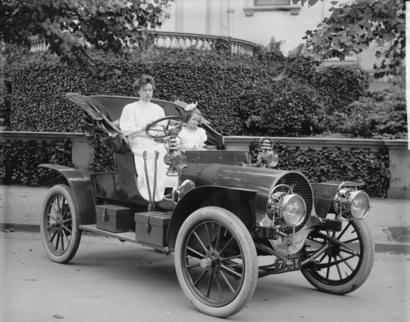
\includegraphics{sample-franklin.png}}
\caption{1907 Franklin Model D roadster. Photograph by Harris \& Ewing,
Inc.~{[}Public domain{]}, via Wikimedia Commons.
(\url{https://goo.gl/VLCRBB}).}
\Description{A woman and a girl in white dresses sit in an open car.}
\end{figure}

Your figures should contain a caption which describes the figure to the
reader.

Figure captions are placed \emph{below} the figure.

Every figure should also have a figure description unless it is purely
decorative. These descriptions convey what's in the image to someone who
cannot see it. They are also used by search engine crawlers for indexing
images, and when images cannot be loaded.

A figure description must be unformatted plain text less than 2000
characters long (including spaces). \textbf{Figure descriptions should
not repeat the figure caption -- their purpose is to capture important
information that is not already provided in the caption or the main text
of the paper.} For figures that convey important and complex new
information, a short text description may not be adequate. More complex
alternative descriptions can be placed in an appendix and referenced in
a short figure description. For example, provide a data table capturing
the information in a bar chart, or a structured list representing a
graph. For additional information regarding how best to write figure
descriptions and why doing this is so important, please see
\url{https://www.acm.org/publications/taps/describing-figures/}.

\hypertarget{the-teaser-figure}{%
\subsection{The ``Teaser Figure''}\label{the-teaser-figure}}

A ``teaser figure'' is an image, or set of images in one figure, that
are placed after all author and affiliation information, and before the
body of the article, spanning the page. If you wish to have such a
figure in your article, place the command immediately before the
\texttt{\textbackslash{}maketitle} command:

\begin{verbatim}
  \begin{teaserfigure}
    \includegraphics[width=\textwidth]{sampleteaser}
    \caption{figure caption}
    \Description{figure description}
  \end{teaserfigure}
\end{verbatim}

\hypertarget{citations-and-bibliographies}{%
\section{Citations and
Bibliographies}\label{citations-and-bibliographies}}

The use of \BibTeX~for the preparation and formatting of one's
references is strongly recommended. Authors' names should be complete
--- use full first names (``Donald E. Knuth'') not initials (``D. E.
Knuth'') --- and the salient identifying features of a reference should
be included: title, year, volume, number, pages, article DOI, etc.

The bibliography is included in your source document with these two
commands, placed just before the
\textbackslash verb\textbar\textbackslash end\{document\}\textbar{}
command:

\begin{verbatim}
  \bibliographystyle{ACM-Reference-Format}
  \bibliography{bibfile}
\end{verbatim}

where ``\texttt{bibfile}'' is the name, without the ``\texttt{.bib}''
suffix, of the \BibTeX~file.

Citations and references are numbered by default. A small number of ACM
publications have citations and references formatted in the ``author
year'' style; for these exceptions, please include this command in the
\textbf{preamble} (before the command
``\texttt{\textbackslash{}begin\{document\}}'') of your \LaTeX~source:

\begin{verbatim}
  \citestyle{acmauthoryear}
\end{verbatim}

Some examples. A paginated journal article \citep{Abril07}, an
enumerated journal article \citep{Cohen07}, a reference to an entire
issue \citep{JCohen96}, a monograph (whole book) \citep{Kosiur01}, a
monograph/whole book in a series (see 2a in spec. document)
\citep{Harel79}, a divisible-book such as an anthology or compilation
\citep{Editor00} followed by the same example, however we only output
the series if the volume number is given \citep{Editor00a} (so
Editor00a's series should NOT be present since it has no vol.~no.), a
chapter in a divisible book \citep{Spector90}, a chapter in a divisible
book in a series \citep{Douglass98}, a multi-volume work as book
\citep{Knuth97}, a couple of articles in a proceedings (of a conference,
symposium, workshop for example) (paginated proceedings article)
\citep[\citet{Hagerup1993}]{Andler79}, a proceedings article with all
possible elements \citep{Smith10}, an example of an enumerated
proceedings article \citep{VanGundy07}, an informally published work
\citep{Harel78}, a couple of preprints
\citep[\citet{AnzarootPBM14}]{Bornmann2019}, a doctoral dissertation
\citep{Clarkson85}, a master's thesis: \citep{anisi03}, an online
document / world wide web resource \citep[\citet{Ablamowicz07},
\citet{Poker06}]{Thornburg01}, a video game (Case 1) \citep{Obama08} and
(Case 2)\citep{Novak03} and \citep{Lee05} and (Case 3) a patent
\citep{JoeScientist001}, work accepted for publication \citep{rous08},
`YYYYb'-test for prolific author \citep{SaeediMEJ10} and
\citep{SaeediJETC10}. Other cites might contain `duplicate' DOI and URLs
(some SIAM articles) \citep{Kirschmer-2010-AEI-1958016-1958018}. Boris /
Barbara Beeton: multi-volume works as books \citep{MR781536} and
\citep{MR781537}. A couple of citations with DOIs:
\citep[\citet{Kirschmer-2010-AEI-1958016-1958018}]{2004-ITE-1009386-1010128}.
Online citations: \citep[\citet{Thornburg01},
\citet{CTANacmart}]{TUGInstmem}. Artifacts: \citep{R} and
\citep{UMassCitations}.

\hypertarget{acknowledgments}{%
\section{Acknowledgments}\label{acknowledgments}}

Identification of funding sources and other support, and thanks to
individuals and groups that assisted in the research and the preparation
of the work should be included in an acknowledgment section, which is
placed just before the reference section in your document.

This section has a special environment:

\begin{verbatim}
  \begin{acks}
  ...
  \end{acks}
\end{verbatim}

so that the information contained therein can be more easily collected
during the article metadata extraction phase, and to ensure consistency
in the spelling of the section heading.

Authors should not prepare this section as a numbered or unnumbered
\texttt{\textbackslash{}section}; please the
``\texttt{\textbackslash{}acks}'' environment.

\hypertarget{appendices}{%
\section{Appendices}\label{appendices}}

If your work needs an appendix, add it before the
``\texttt{\textbackslash{}end\{document\}}'' command at the conclusion
of your source document.

Start the appendix with the ``\texttt{appendix}'' command:

\begin{verbatim}
  \appendix
\end{verbatim}

and note that in the appendix, sections are lettered, not numbered. This
document has two appendices, demonstrating the section and subsection
identification method.

\hypertarget{multi-language-papers}{%
\section{Multi-language papers}\label{multi-language-papers}}

Papers may be written in languages other than English or include titles,
subtitles, keywords and abstracts in different languages (as a rule, a
paper in a language other than English should include an English title
and an English abstract). Use \texttt{language=...} for every language
used in the paper. The last language indicated is the main language of
the paper. For example, a French paper with additional titles and
abstracts in English and German may start with the following command

\begin{verbatim}
  \documentclass[sigconf, language=english, language=german,
                 language=french]{acmart}
\end{verbatim}

The title, subtitle, keywords and abstract will be typeset in the main
language of the paper. The commands
\texttt{\textbackslash{}translatedXXX}, \texttt{XXX} being
\texttt{title}, \texttt{subtitle} and \texttt{keywords}, can be used to
set these elements in the other languages. The environment
\texttt{translatedabstract} is used to set the translation of the
abstract. These commands and environment have a mandatory first
argument: the language of the second argument. See
\texttt{sample-sigconf-i13n.tex} file for examples of their usage.

\hypertarget{sigchi-extended-abstracts}{%
\section{SIGCHI Extended Abstracts}\label{sigchi-extended-abstracts}}

The ``\texttt{sigchi-a}'' template style (available only in \LaTeX~and
not in Word) produces a landscape-orientation formatted article, with a
wide left margin. Three environments are available for use with the
``\texttt{sigchi-a}'' template style, and produce formatted output in
the margin:

\begin{itemize}
\tightlist
\item
  \textbf{\texttt{sidebar}}: Place formatted text in the margin.
\item
  \textbf{\texttt{marginfigure}}: Place a figure in the margin.
\item
  \textbf{\texttt{margintable}}: Place a table in the margin.
\end{itemize}

\begin{acks}
To Robert, for the bagels and explaining CMYK and color spaces.
\end{acks}

\bibliographystyle{ACM-Reference-Format}
\bibliography{bibliography.bib}

\hypertarget{refs}{}
\begin{CSLReferences}{0}{0}
\end{CSLReferences}

\appendix

\hypertarget{research-methods}{%
\section{Research Methods}\label{research-methods}}

\hypertarget{part-one}{%
\subsection{Part One}\label{part-one}}

Lorem ipsum dolor sit amet, consectetur adipiscing elit. Morbi
malesuada, quam in pulvinar varius, metus nunc fermentum urna, id
sollicitudin purus odio sit amet enim. Aliquam ullamcorper eu ipsum vel
mollis. Curabitur quis dictum nisl. Phasellus vel semper risus, et
lacinia dolor. Integer ultricies commodo sem nec semper.

\hypertarget{part-two}{%
\subsection{Part Two}\label{part-two}}

Etiam commodo feugiat nisl pulvinar pellentesque. Etiam auctor sodales
ligula, non varius nibh pulvinar semper. Suspendisse nec lectus non
ipsum convallis congue hendrerit vitae sapien. Donec at laoreet eros.
Vivamus non purus placerat, scelerisque diam eu, cursus ante. Etiam
aliquam tortor auctor efficitur mattis.

\hypertarget{online-resources}{%
\section{Online Resources}\label{online-resources}}

Nam id fermentum dui. Suspendisse sagittis tortor a nulla mollis, in
pulvinar ex pretium. Sed interdum orci quis metus euismod, et sagittis
enim maximus. Vestibulum gravida massa ut felis suscipit congue. Quisque
mattis elit a risus ultrices commodo venenatis eget dui. Etiam sagittis
eleifend elementum.

Nam interdum magna at lectus dignissim, ac dignissim lorem rhoncus.
Maecenas eu arcu ac neque placerat aliquam. Nunc pulvinar massa et
mattis lacinia.

%% begin pandoc before-bib
%% end pandoc before-bib
%% begin pandoc biblio
%% end pandoc biblio
%% begin pandoc include-after
%% end pandoc include-after
%% begin pandoc after-body
%% end pandoc after-body

\end{document}
\endinput
%%
%% End of file `sample-manuscript.tex'.
